
	The HIV internal dynamics is the interaction between the HIV-1 virus and the immune system. 
\citeauthor*{Dalal2008} in \cite{Dalal2008} propose a compartmental stochastic model, which capture the interaction 
between CD-4 for cells and HVI-1 virus. They perturbed  with noise the per capita rate parameters of the three kind of 
populations described by
\begin{align}\label{eqn:HIVDynamics}
	\frac{dy_1(t)}{dt} &=
		\left(
			\lambda -\delta y_1(t) - (1 - \gamma) \beta y_1(t) y_3(t)
		\right),
		\notag \\
	\frac{dy_2(t)}{dt} &= 
		\left(
			(1- \gamma) \beta y_1(t) y_3(t) - a y_2(t) 
		\right),
	\\
	\frac{dy_3(t)}{dt} & = 
		\left(
			(1 - \eta) N a y_2(t) 
			-u y_3(t)
			-(1 - \gamma ) \beta y_1(t) y_3(t) 
		\right).
	\notag
\end{align}
Where:
\begin{table}[h!]
	\begin{center}
	\begin{tabular}{rl}
		$y_1(t)$ &				is the concentration of uninfected cells;\\ 
		$y_2(t)$ &				is the concentration of infected cells; \\
		$y_3(t)$ &				is the concentration of virus particles;\\
		$(1 - \gamma)$ &	is the reverse transcriptase inhibitor drug effect;\\
		$(1 -\eta)$ &			is the protease inhibitor drug effect; \\
		$\lambda$ &				is the total rate of production of healthy cells per unit time;\\
		$\delta$ &				is the per capita death rate of healthy cells;\\
		$\beta$ &					is the transmission coefficient between uninfected cells and infective virus particles;\\
		$a$ & 						is the per capita death rate of infected cells;\\
		$N$ &							is the average number of infective virus particles produced by an infected\\ 
				&							cell in the absence of the Highly Active Antiretroviral Treatment (HAART)\\
				&							during its entire infectious lifetime; \\
		$u$&							is the per capita death rate of infective virus particles.
	\end{tabular}
	\end{center}
\end{table}

	Because rates of death for both, CD-4 cells and HIV-1 virus are affected by great amount of biological complex 
mechanisms, the authors introduce randomness into the model by replacing the parameters $\delta$, $a$, and $u$ by
$\delta \to \delta+ \sigma_1 dW^{(1)}_t$,
$a \to a + \sigma_2 dW^{(1)}_t$, and
$u \to u + \sigma_2 dW^{(2)}_t$,
where $W^{(1)}_t$, $W^{(2)}_t$ are independent Brownian motions with intensities $\sigma_1$, $\sigma_2$.
They obtain the following system of stochastic differential equations
\begin{align}\label{eqn:StochasticHIVDynamics}
	dy_1(t) &=
		\left(
			\lambda -\delta y_1(t) - (1 - \gamma) \beta y_1(t) y_3(t)
		\right)dt,
		-\sigma_1 y_1(t) dW^{(1)}_t, 
		\notag \\
	dy_2(t) &= 
		\left(
			(1- \gamma) \beta y_1(t) y_3(t) - a y_2(t) 
		\right)dt,
		-\sigma_1 y_2(t) dW^{(1)}_t, 
	\\
	dy_3(t) & = 
	\left(
		(1 - \eta) N a y_2(t) 
		-u y_3(t)
		-(1 - \gamma ) \beta y_1(t) y_3(t) 
	\right)dt
	- \sigma_2 y_3(t) dW^{(2)}_t.
	\notag
\end{align}

	\citeauthor{Dalal2008} give suitable conditions to assure that  the number of infected cells and virus particles tend
asymptotically to zero almost surely \cite[Thm. 5.1]{Dalal2008}. They support their analytical results by the 
simulation of SDE 
\eqref{eqn:StochasticHIVDynamics}. All the parameters values that they used, have been taken from published 
literature \cite{Bonhoeffer1997, Callaway2002, Nelson2000, Nowak1997}.

	Using the following \SM scheme
\begin{align}\label{eqn:SteklovSchemMaoAdis2}
	X^{(j)}_{k+1}
			&=
			\left(
				X_k^{(j)} + 
				\frac{b_j }{a_j}
			\right) 
			\exp\left(
					a_j h
				\right) - \frac{b_j}{a_j}
		+ g^{(j)}(X_k) \Delta W^{(j)}_k, \qquad j \in \{1,2,3\} \notag 
		\\
	g^{(1)}(X_k) &=- \sigma_1 X_{k}^{(1)},  \qquad
	g^{(2)}(X_k)= - \sigma_1 X_{k}^{(2)}, \qquad
	g^{(3)}(X_k)= - \sigma_2 X_{k}^{(3)}, \notag
\end{align}
\begin{alignat}{2}%\label{eqn:SteklovHIVDynamicsCoef}	
	a_{1} &= 
		-\left(
			\delta + (1 - \gamma) \beta X_{k}^{(3)}
		\right),
	& \qquad
	b_1 &= \lambda, \notag
	\\
	a_{2} &= -a,
	& \qquad
	b_2 &=
		(1-\gamma) \beta X_{k+1}^{(1)} X_{k}^{(3)}, 
\\
	a_{3} &= 
		-
	\left(
			u + (1- \gamma) \beta X_{k+1}^{(1)}
		\right),
	& \qquad
	b_{3} &= 
		\left(
			1 - \eta 
		\right)
		N a X_{k+1}^{(3)}, \notag
\end{alignat}
we contrast the approximations of SDE \eqref{eqn:StochasticHIVDynamics} with the corresponding EM method.
In \Cref{fig:StochasticHIVDynamicsPaths} utilizing a step-size $h=\num{0.5}$, we observe how the EM method diverge,
while the \SM obeys the EM numerical realization of the solution with a very small ($h=\num{0.0005}$) step-size.
\begin{figure}[htb]
	\begin{center}
		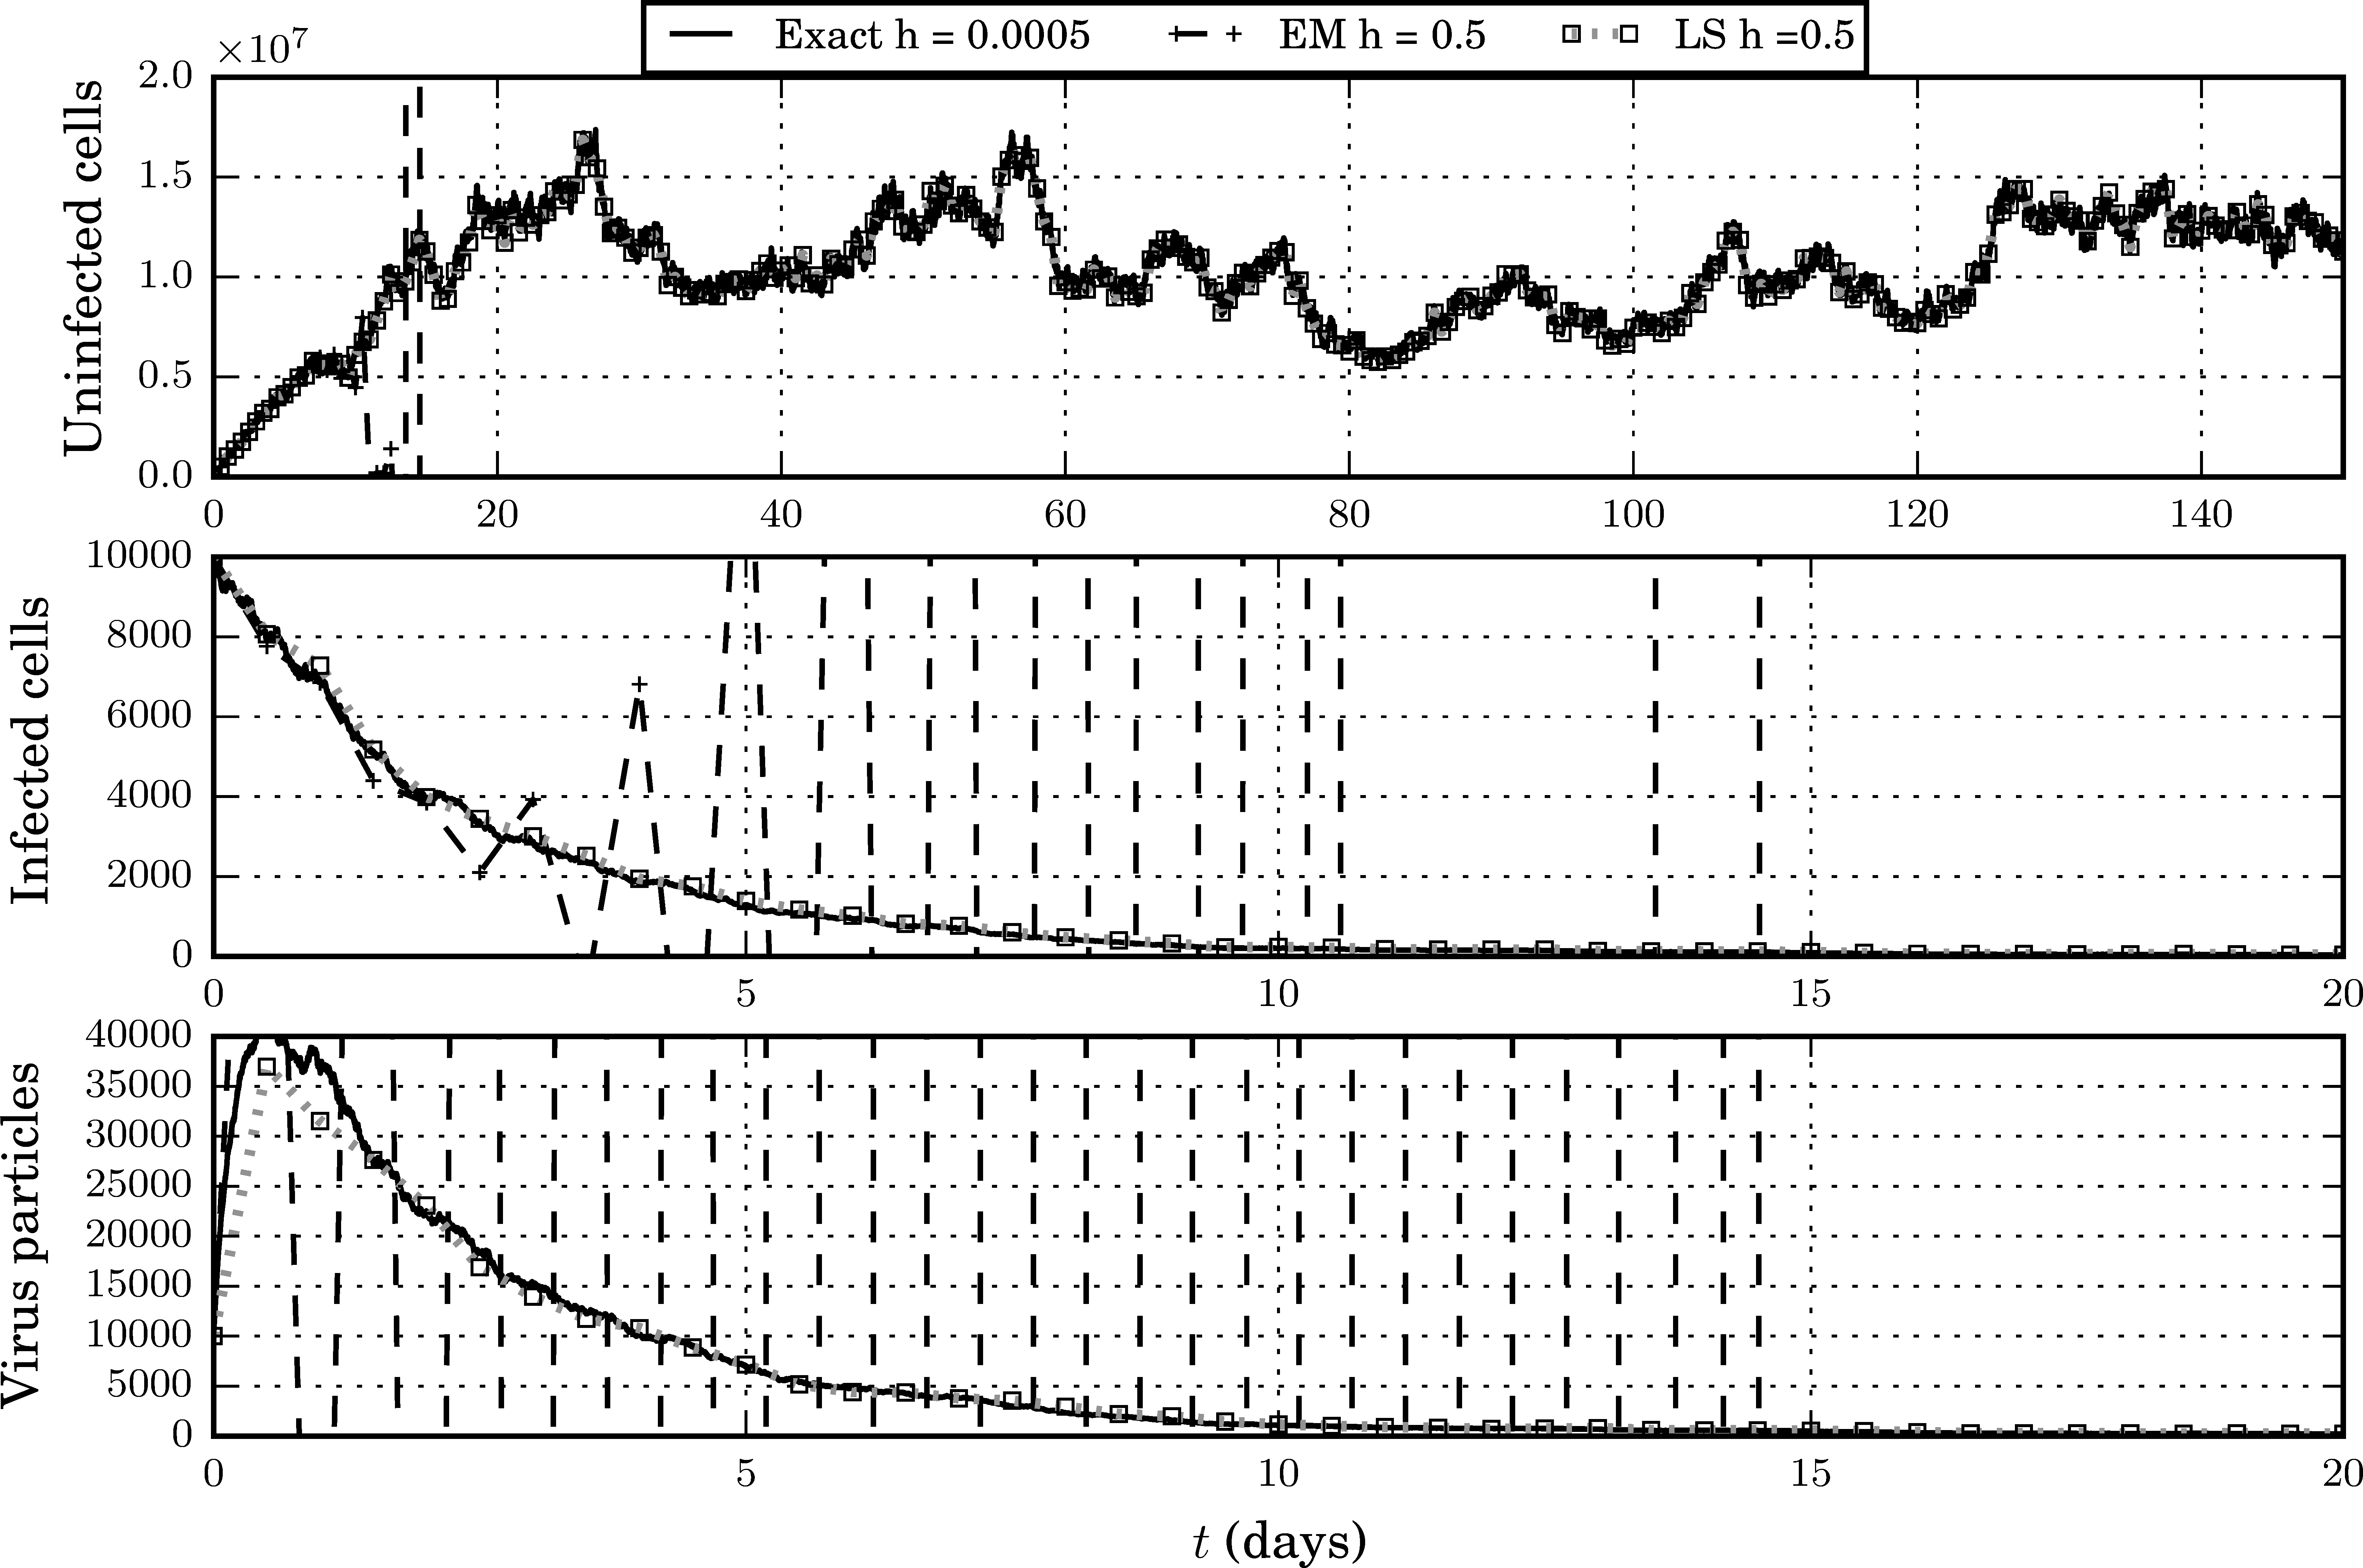
\includegraphics{./papers/paperB/figures/InternalHIVDynamics5e-1.png}
		\caption{
			Likening between EM and SM schemes for SDE \eqref{eqn:StochasticHIVDynamics} with
			$\gamma = \num{0.5}$,
			$\eta = \num{0.5}$,
			$\lambda = \SI{1e6}{\per\cubic\deci\meter\per\day}$,
			$\delta = \SI{0.1}{\per\day}$,
			$\beta = \SI{1e-8}{\cubic\deci\meter\per\day}$,
			$a = \SI{0.5}{\per \day}$,
			$N = \SI{100}{per cell}$,
			$u = \SI{5}{\per\day} $,
			$\sigma_1 = \num{0.1}$,
			$\sigma_2 = \num{0.1} $,
			$X_0 = (\SI{10000}{\per\cubic\deci\meter}, \SI{10000}{\per\cubic\deci\meter}, 
			\SI{10000}{\per\cubic\deci\meter})^T$,
			$h=\num{0.5}$.
			Here the exact solution means a EM simulation
			with the same parameters but with a step-size $h=\num{1e-5}$.
		}
		\label{fig:StochasticHIVDynamicsPaths}
	\end{center}
\end{figure}

